% ----------------------------------------------------------
% Introdução 
% Capítulo sem numeração, mas presente no Sumário
% ----------------------------------------------------------

\chapter[Introdução]{Introdução}
\addcontentsline{toc}{chapter}{Introdução}

O avanço da tecnologia está relacionado diretamente com a demanda de energia elétrica. A inserção de cada vez mais aparelhos eletrônicos, automatização de antigos processos e criação de novas tecnologias como carros elétricos implica um aumento constante na demanda de energia elétrica. “Em 2030, estima-se um consumo de energia elétrica entre 950 e 1.250 TWh/ano, sendo que o consumo atual situa-se em torno de 405 TWh” (ANEEL, Atlas de Energia Elétrica no Brasil 2006).

A perspectiva do aumento da demanda faz com que seja necessário um investimento maior no setor energético, de acordo com Bronzati essa grande diferença entre a demanda de 2030 que a demanda atual “exigirá investimentos pesados na expansão da oferta de energia elétrica. No caso deste fornecimento ser realizado por usinas hidrelétricas, mesmo com uma instalação adicional de 120 mil MW, o que eleva para 80\% o uso do potencial, ainda assim poderia não ser suficiente para atender a demanda em 2030.

Mesmo com o aumento do uso do potencial hídrico, é notável que há uma necessidade de diversificação da matriz energética, onde essa diversificação deve buscar a inserção de fontes renováveis. Pequenas Centrais Hidrelétricas representam se mostram uma alternativa muito viável, possibilitando uma geração próxima da carga, um impacto ambiental menor que as grandes usinas, além de um maior custo.

\section{Objetivo}\label{sec:obj}
Projetar uma PCH e realizar seu estudo de viabilidade.

\subsection{Objetivos Específicos}
\begin{itemize}
\item Escolher uma bacia hidrográfica que não possua nenhuma usina instalada;
\item Determinar a potência gerada ao ano;
\item Determinar as máquinas utilizadas;
\item Descrever o maquinário e estruturas auxiliares;
\item Realizar o estudo de payback;
\item Avaliar o projeto técnico e financeiramente;

\end{itemize}

\section{Fundamentação teórica}
\subsection{Pequena Central Hidrelétrica}
Segundo a Aneel, Pequenas Centrais Hidrelétricas (PCH) são os empreendimentos hidrelétricos com potência superior a $1.000 kW$ e igual ou inferior a $30.000 kW$ e com área total de reservatório igual ou inferior a $3,0 km^2$. As PChs são normalmente instaladas em rios que possuam desníveis significativos que possam gerar potência hidráulica suficiente para movimentar as turbinas. Por operarem normalmente a fio d’água e serem em geral instalações de menor porte ao comparar com as usinas hidrelétricas elas acabam resultando em um menor impacto ambiental.

Conforme a Eletrobrás as PCHS são classificadas quanto sua capacidade de regularização por: a fio d’água, acumulação, com regulação mensal do reservatório ou acumulação com regulação diária do reservatório. Elas podem ser classificadas também quanto sua potência instalada quanto a queda do projeto, conforme mostra o quadro abaixo.

\begin{figure}[h]
	\centering
	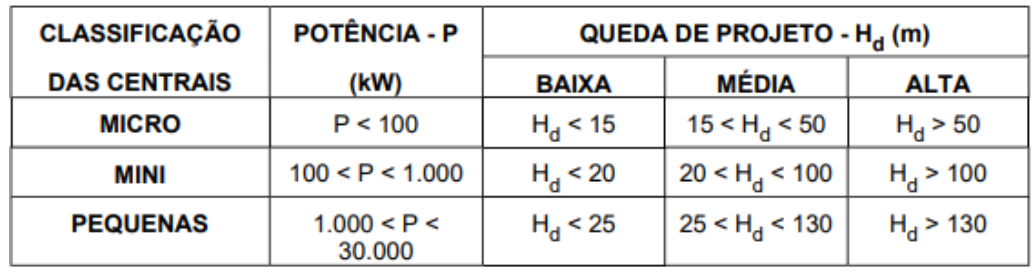
\includegraphics[width=1\textwidth]{quadro_tipos.png}
	\caption{Quadro de classificação dos tipos de PCH}
	\label{fig:tcp_packet}
	\source{Manual da Eletrobrás}
\end{figure}

\subsection{Tipos de PCH de acordo com a capacidade de regularização}
\subsubsection{A fio d’água} 

Tipo de PCH mais adequada para quando as vazões de estiagem do rio são maiores que a descarga necessária para potência a ser instalada para suprir a demanda.
Esse tipo de projeto é mais simples, pois não requer estudos de regularização de vazões e estudos de sazonalidade de carga elétrica do consumidor.

\subsubsection{Acumulação diaria com regularização diária do reservatório }

PCH utilizada em situações onde as vazões de estiagem do rio são inferiores a necessária para fornecer a potência requerida, por isso é necessário a acumulação. Nesse caso, tem que haver um estudo de qual volume d’água precisa ser acumulado diariamente para suprir a demanda.

\subsubsection{Acumulação diaria com regularização mensal do reservatório }

Semelhante ao tipo de PCH anterior, porém com a diferença do tempo de regularização, oriundo do estudo prévio do rio, que fornece informações dos estudos mensais do rio, e não diário.

Conhecendo os diferentes tipos de usina, pode-se analisar qual se adequa mais para o uso da a implementação do referido artigo, que no caso seria a PCH de acumulação diária com regularização diária do reservatório, pois os dados coletados do rio que vai ser apresentado posteriormente foram coletados com um espaço amostral diário.
